%%%%%%%%%%%%%%%%%%%%%%%%%%%%%%%%%%%%%%%%%%%%%%%%%%%%%%%%%%%%%%%%%%%%%%%%%%%%%%%%
% CS 2640 . Final Report (USENIX format) . Mira Yu
%%%%%%%%%%%%%%%%%%%%%%%%%%%%%%%%%%%%%%%%%%%%%%%%%%%%%%%%%%%%%%%%%%%%%%%%%%%%%%%%

\documentclass[letterpaper,twocolumn,10pt]{article}
\usepackage{usenix-2020-09}

\usepackage{booktabs}
\usepackage{tabularx}
\usepackage{enumitem}
\usepackage{amsmath}
\usepackage{amssymb}
\usepackage{graphicx}
\usepackage{subcaption}

\newcommand{\code}[1]{\texttt{\small #1}}

%-------------------------------------------------------------------------------
\begin{document}
%-------------------------------------------------------------------------------

\date{}

\title{\Large \bf Cache Eviction on Public-Records APIs:\\
Workload Shape and Cost Attribution Decide the Policy}

\author{
{\rm Mira Yu}\\
Harvard University \\
CS 2640: Modern Storage Systems
}

\maketitle

%-------------------------------------------------------------------------------
\begin{abstract}
%-------------------------------------------------------------------------------
Which cache eviction policy wins on public-records APIs? The
honest answer depends on what the operator is paying for.
Public-records APIs (Congress.gov, CourtListener) are rate-limited
at the origin ($\sim 5{,}000$ req/hr), have no per-byte charge,
span $335\times$ size variance in a single namespace, and are
TTFB-dominated ($\sim 358$\,ms p50). Object-miss is the
deployment cost; byte-miss is not. That attribution flips
the post-2020 ``size-aware-is-dead'' trend
(Caffeine~\cite{caffeine2024}, S3-FIFO~\cite{yang2023fifo},
SIEVE~\cite{zhang2024sieve}).

On two real traces with 5-seed sweeps over four $\alpha$, four cache
fractions, and ten policies (LRU, FIFO, CLOCK, S3-FIFO, SIEVE,
W-TinyLFU, GDSF, GDSF-Cost, LHD-Lite, LHD-Full), the object-miss
winner depends on workload shape. \textbf{GDSF wins on Court
(heavy-tail size)} at $\code{cache\_frac} \geq 0.01$, $3$--$9$\,pp
over W-TinyLFU at $0.01$ and $4$--$21$\,pp at $0.05$; W-TinyLFU
takes smaller caches ($\leq 0.005$). \textbf{LHD-Full wins on
Congress (light-tail size)} at $\alpha \leq 0.8$, where its
residual-reuse-distance signal beats GDSF's size-priority. Three
controls narrow the SIEVE-vs.-W-TinyLFU gap on Court to size-outlier
rejection, not frequency-gradient capture. LHD-Full is
Pareto-dominated by the GDSF--W-TinyLFU convex hull on Court ($7/8$
deployment-relevant cells) but anchors the object-miss frontier on
Congress at low $\alpha$.

For byte-priced backends (S3 egress) the verdict flips to W-TinyLFU
on Court and SIEVE on Congress: same measurements, opposite winner.
The metric you choose is the policy you choose because choosing one
without naming the cost model chooses both implicitly.
\end{abstract}

%-------------------------------------------------------------------------------
% Hero figure (full-width, two-column-spanning)
%-------------------------------------------------------------------------------
\begin{figure*}[t]
\centering
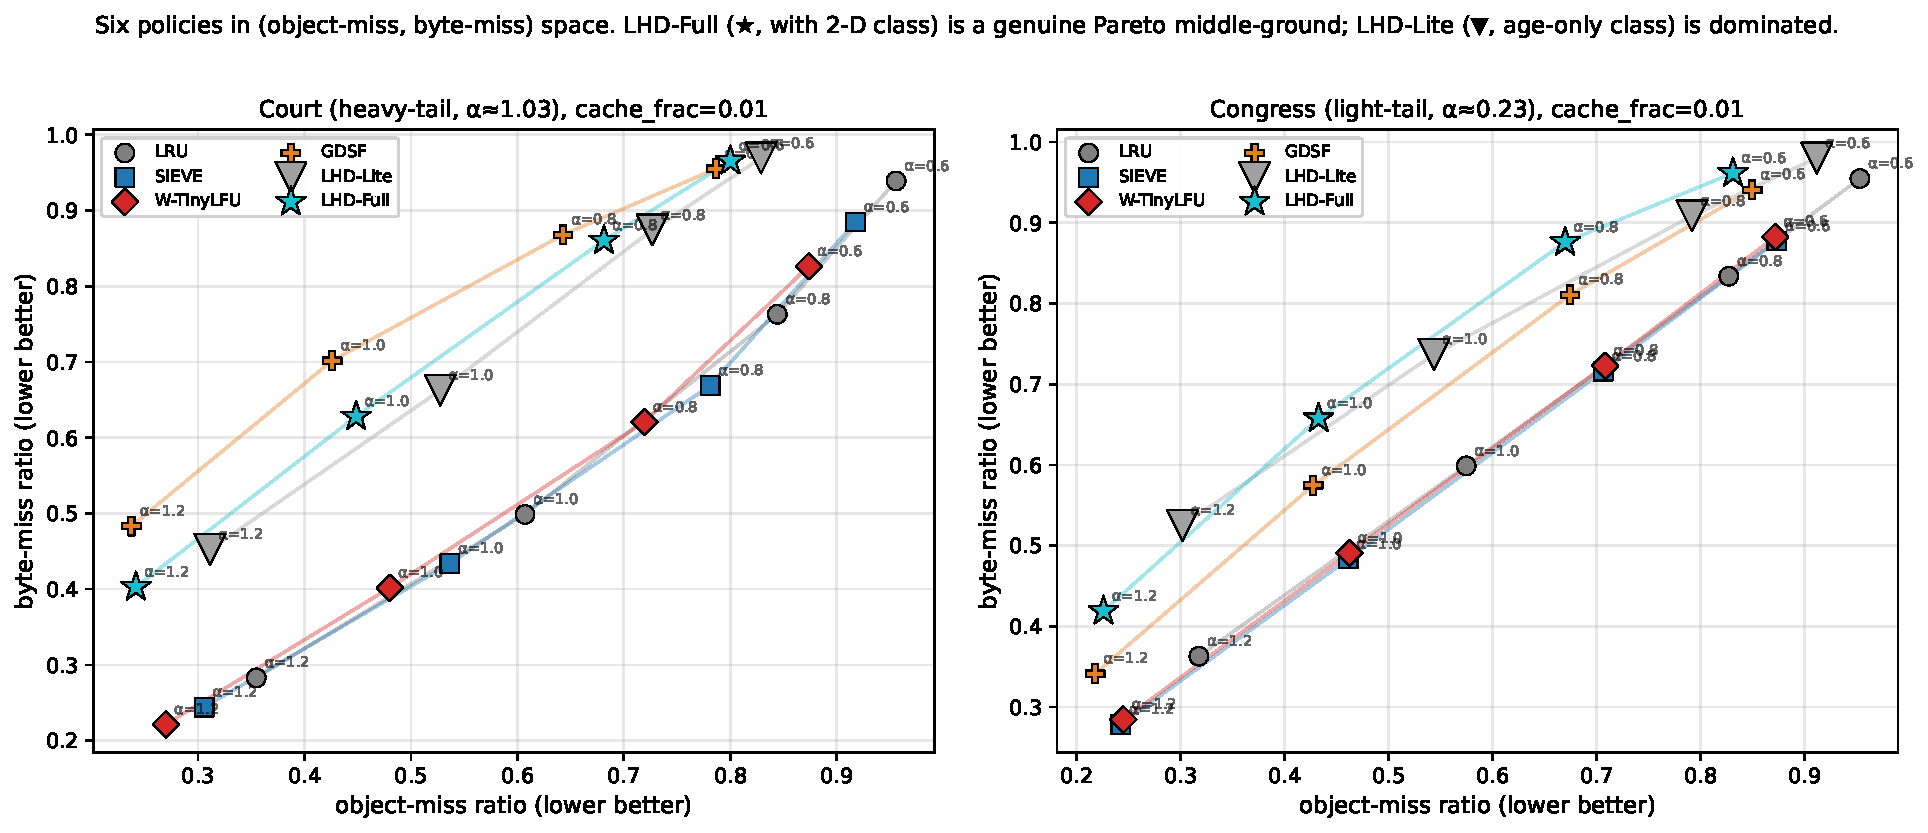
\includegraphics[width=0.75\textwidth]{figures/obj_vs_byte_lhdfull.pdf}
\caption{Six policies in (object-miss, byte-miss) space at
$\code{cache\_frac} = 0.01$, four $\alpha$ overlays per workload.
GDSF anchors the low-object-miss frontier; W-TinyLFU anchors the
low-byte-miss frontier, so the two are not co-optimizable. Which axis
is the deployment cost depends on who pays
(\S\ref{sec:weighted}).}
\label{fig:headline}
\end{figure*}

%-------------------------------------------------------------------------------
\section{Introduction}\label{sec:intro}
%-------------------------------------------------------------------------------

The TinyLFU paper~\cite{einziger2017tinylfu} argued that frequency
tracking would dominate recency-only eviction. The post-2020
literature (Caffeine~\cite{caffeine2024}, S3-FIFO~\cite{yang2023fifo},
SIEVE~\cite{zhang2024sieve}) has implicitly accepted that framing while
moving away from size-aware policies; the broader 2000s adaptive-cache
work (ARC~\cite{megiddo2003arc}) is recency+frequency, also not
size-aware. I collected two real public-records API traces
(Congress.gov, CourtListener), ran a 5-seed comparison of ten policies
including GDSF~\cite{cherkasova1998gdsf} (the canonical
size-aware-with-frequency policy that dropped out of the modern
comparison set) and LHD~\cite{beckmann2018lhd}, and tabulated
\emph{both} object-miss and byte-miss for every cell. The headline
result (GDSF wins object-miss on Court at deployment-relevant cache
fractions; LHD-Full wins on Congress at low $\alpha$; W-TinyLFU wins
byte-miss universally on Court) becomes obvious only after attributing
cost workload-class-specifically (\S\ref{sec:weighted}) rather than
picking a metric a priori.

\paragraph{Why public-records APIs are a distinct workload class.}
Most cache-policy benchmark papers treat ``the workload'' as
interchangeable Zipf parameters; what differs across CDN, key-value,
and storage benchmarks is mostly $\alpha$ and the size distribution.
Public-records APIs are different in five concrete ways that change
the answer:

\begin{enumerate}[leftmargin=*,itemsep=1pt,topsep=2pt]
  \item \textbf{The origin is rate-limited, not bandwidth-billed.}
    Congress.gov and CourtListener publish hard quotas
    ($\sim 5{,}000$ req/hr); breaches return 429s rather than
    overage charges. The operator's binding cost is requests
    issued to origin, not bytes transferred. This collapses the
    object-miss/byte-miss tradeoff in favor of object-miss (\S\ref{sec:weighted}).
  \item \textbf{Heavy size variance inside one namespace.}
    A single CourtListener \texttt{/opinion/} prefix returns both
    $200$\,B metadata stubs and $462$\,KB full-text opinions
    ($335\times$ ratio, Table~\ref{tab:workload}). Most cache
    benchmark traces are size-uniform (key-value) or size-binned
    (video chunks). The same key prefix in this workload spans the
    full size range.
  \item \textbf{TTFB-dominated origin response} ($358$\,ms combined
    $p_{50}$). Cost of a miss is whether-you-hit, not transfer time
    making latency $\approx$ object-miss $\times \, L_{\text{origin}}$
    tight up to $\sim 100$\,KB sizes (\S\ref{sec:weighted}).
  \item \textbf{The cache is the only operator lever.} A private
    operator cannot scale, renegotiate, or bypass the public origin, and
    cache hit rate directly bounds simultaneous users.
  \item \textbf{Catalog-then-deepdive access.} Sessions enumerate
    catalogs (many low-freq items) then drill into specific records
    (few high-freq items), giving heavy-tailed frequency
    ($\alpha \approx 1.03$ on Court).
\end{enumerate}

Traits (1)+(3) make object-miss the unique cost; (2) makes size-aware
admission valuable; (4) makes the result deployable rather than
academic; (5) gives the high-$\alpha$ structure caching needs to
work at all. None of these are unique individually (CDN
traces have heavy tails, key-value caches have rate-limit-like
SLOs), so the combination is important.

\paragraph{Trace caveat.} Both real traces are dominated
by one-hit wonders ($\S$\ref{sec:methodology}), so the policy
comparison runs against a controlled Zipf overlay on the real key set
(real keys, real sizes, resampled popularity ranks). The
key/size distributions carry the workload-class signal and the
popularity is the controlled variable.

%-------------------------------------------------------------------------------
\section{Related Work}\label{sec:related}
%-------------------------------------------------------------------------------

\paragraph{Modern cache eviction.} The post-2020 wave of
S3-FIFO~\cite{yang2023fifo}, SIEVE~\cite{zhang2024sieve}, and
Caffeine's W-TinyLFU~\cite{caffeine2024} converges on
recency/frequency signals over size-aware admission, building on
TinyLFU~\cite{einziger2017tinylfu} and the earlier
ARC~\cite{megiddo2003arc}. Each evaluation implicitly fixes its cost
model by metric choice: SIEVE and S3-FIFO target object-miss for
KV/web; LHD~\cite{beckmann2018lhd} targets byte-miss for CDN.
GDSF~\cite{cherkasova1998gdsf} sits outside this trend and has not
appeared in the post-2020 comparison set, which is what motivates
revisiting it under workload-class-specific cost attribution.

\paragraph{Trace characterization.} Most published cache benchmarks
treat workload as interchangeable Zipf parameters with optional size
binning. CDN traces (Akamai, Wikipedia) are heavy-tailed in
popularity but typically size-binned by content type; KV traces
(Twitter, Memcached production) are size-uniform within a namespace.
Heavy size variance within a single key prefix, 
$335\times$ on a single CourtListener URL prefix, is rare in the
published trace literature, and is the structural feature that drives
GDSF's win here.

\paragraph{Cache simulators.} The CMU CORGI/LHD reference
implementation is the canonical LHD codebase; this paper validates
against the LHD paper's Memcached comparison
(\S\ref{sec:methodology}, $13$--$18$\,pp over LRU on a synth-faithful
trace) but does not yet run a byte-for-byte CORGI comparison —
flagged in \S\ref{sec:conclusion}.
SHARDS~\cite{waldspurger2015shards} provides MRC sampling, used here
for self-convergence validation (\S\ref{sec:ablations}).

\paragraph{Cost-aware evaluation.} GDSF~\cite{cherkasova1998gdsf} is
itself cost-aware (priority $H = f \cdot c / s + L$); the cost-aware
literature historically jointly optimizes hit-rate and bandwidth for
web proxies. This paper's contribution is not new policy design but
cost-attribution-driven policy \emph{selection}: when the operator's
binding cost is requests-to-origin (rate-limited APIs), the right
policy differs from the byte-priced default, and the choice should be
named not silent.

\paragraph{API gateway caching.} Production API gateways (Kong,
Cloudflare Workers, AWS API Gateway) ship LRU/TTL by default;
cache-policy choice for rate-limited public APIs is largely
undocumented in the academic literature, which is the gap this report
addresses.

%-------------------------------------------------------------------------------
\section{Workloads and Methodology}\label{sec:methodology}
%-------------------------------------------------------------------------------

\begin{figure*}[t]
\centering
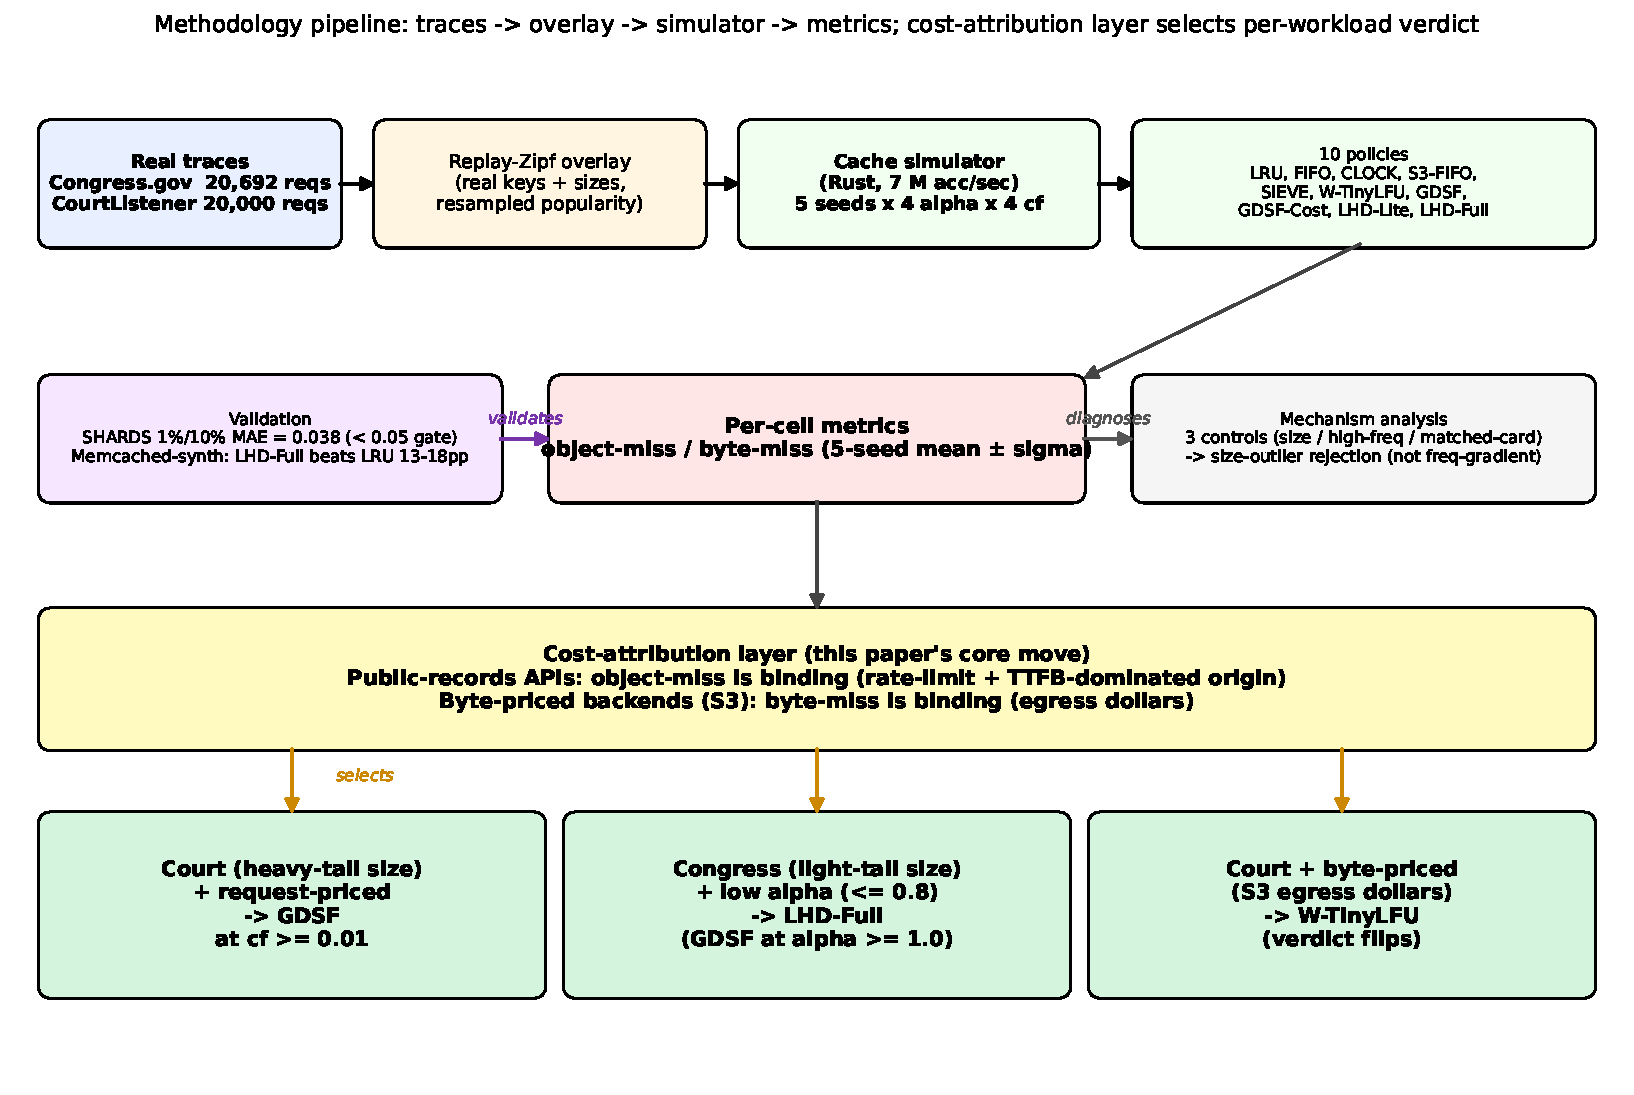
\includegraphics[width=0.92\textwidth]{figures/methodology_diagram.pdf}
\caption{Methodology pipeline. Real traces feed a Zipf-overlay
preprocessor; a Rust simulator runs ten policies under a $5
\times 4 \times 4$ sweep, validated by SHARDS and a
Memcached-faithful synth. The cost-attribution layer selects a
deployment verdict from the same per-cell metrics.}
\label{fig:methodology}
\end{figure*}

\begin{table*}[t]
\centering
\footnotesize
\renewcommand{\arraystretch}{0.95}
\begin{tabularx}{\textwidth}{@{}lXX@{}}
\toprule
\textbf{Metric} & \textbf{Congress.gov} & \textbf{CourtListener} \\
\midrule
Total requests / unique keys & $20{,}692$ / $18{,}970$ & $20{,}000$ / $15{,}018$ \\
Zipf $\alpha$ (Clauset MLE)~\cite{clauset2009powerlaw} & $0.231$ & $1.028$ \\
One-hit-wonder ratio (10\% rolling window) & $0.989$ & $1.000$ \\
Median / max object size (B) & $231$ / $6{,}700$ & $1{,}381$ / $\mathbf{462{,}490}$ \\
Max / median ratio  & $29\times$ & $\mathbf{335\times}$ \\
Origin $p_{50}$ response (ms) & $321$ & $383$ \\
Working set (bytes) & $14.5$\,MB & $59.6$\,MB \\
\bottomrule
\end{tabularx}
\caption{Side-by-side trace characterization. The bold rows (Court's
high $\alpha$ and $335\times$ size ratio) drive the policy gap in
$\S$\ref{sec:gdsf}--$\S$\ref{sec:mechanism}.}
\label{tab:workload}
\end{table*}

\paragraph{Where each policy appears.} Focal object-miss/byte-miss sweep
(Table~\ref{tab:focal-court}): SIEVE, W-TinyLFU, GDSF, LHD-Full.
Hero figure adds LRU and LHD-Lite. \S\ref{sec:ablations} tests
S3-FIFO, SIEVE$\pm$visited-bit, W-TinyLFU$\pm$Doorkeeper. FIFO,
CLOCK, and GDSF-Cost run in the synthetic $1$\,M-request sweep
behind \S\ref{sec:mechanism}.

\paragraph{Trace collection.} Congress.gov v3 REST at $1.2$\,s pacing
sweeping \texttt{/bill/}, \texttt{/amendment/}, \texttt{/vote/}.
CourtListener REST v4 at $0.8$\,s base $+ 0.4$\,s jitter, $80/20$
metadata vs full-text. Both are client-generated random queries against
cataloged keys; no production user-traffic capture exists.
Rate-limit-bounded at $\sim 4500$/hour and $\sim 5000$/hour respectively;
$100$\,K-scale collection would be $\sim 22$\,hours per API.

\paragraph{Replay-Zipf overlay.} The OHW dominance ($\geq 0.989$) on
both raw traces means a direct replay collapses every policy to FIFO.
I overlay a controlled Zipf popularity distribution on the real key
set (real keys, real sizes, resampled popularity ranks). The
distribution is the controlled variable; the keys and sizes are real.

\paragraph{GDSF / LHD implementation.}
GDSF~\cite{cherkasova1998gdsf} maintains $H = f \cdot c / s + L$ per
item, evicting $\arg\min H$ via $O(\log n)$ min-heap with lazy stale-
entry deletion. I tested both unit-cost ($c=1$) and an empirical
linear cost fit ($c = 530 + 0.00254 \cdot \text{size}_{\text{B}}$);
results agree within $0.5$\,pp because size variation ($335\times$)
dominates cost variation ($3.2\times$). I implement
LHD~\cite{beckmann2018lhd} per NSDI'18 \S 4 in two versions:
\textbf{LHD-Lite} (single-class, age only) and \textbf{LHD-Full}
(2-D classes age$\times$freq, $16$ log-spaced age bins $\times\,4$
freq bins, EWMA-decayed histograms, $K=64$ candidate sampling).
LHD-Lite is dominated by every modern policy; LHD-Full is what wins
on Congress at low $\alpha$. \textbf{Implementation validation:} on
a Memcached-faithful synth ($200$K objects, $\alpha=0.9$, log-normal
sizes $\mu=6.5,\sigma=1.5$), LHD-Full beats LRU by $13$--$18$\,pp
and matches GDSF within $\pm 0.5$\,pp, reproducing NSDI'18's primary
claim. Court Pareto-domination by GDSF (\S\ref{sec:weighted}) is
therefore workload-class divergence, not implementation gap.

%-------------------------------------------------------------------------------
\section{Per-Metric Results}\label{sec:gdsf}
%-------------------------------------------------------------------------------

Focal sweep: $5$ seeds $\times$ $4$ alphas $\times$ $4$ cache fractions,
both workloads, both metrics. All 16 Court cells in
Table~\ref{tab:focal-court}; Congress slice in
Table~\ref{tab:focal-congress}.

\begin{table*}[t]
\centering
\footnotesize
\renewcommand{\arraystretch}{0.95}
\begin{tabularx}{\textwidth}{@{}llXXXX@{}}
\toprule
$\alpha$ & cf & SIEVE & W-TinyLFU & GDSF & LHD-Full \\
\midrule
$0.6$ & $0.001$ & $0.992 / 0.995$ & $\mathbf{0.942}$ / $\mathbf{0.975}$ & $0.988 / 0.996$ & $0.987 / 0.996$ \\
$0.6$ & $0.005$ & $0.960 / 0.970$ & $\mathbf{0.891}$ / $\mathbf{0.936}$ & $0.921 / 0.979$ & $0.918 / 0.980$ \\
$0.6$ & $0.01$  & $0.918 / 0.885$ & $0.874 / \mathbf{0.826}$            & $\mathbf{0.787}$ / $0.955$ & $0.800 / 0.966$ \\
$0.6$ & $0.05$  & $0.747 / 0.700$ & $0.730 / \mathbf{0.699}$            & $\mathbf{0.518}$ / $0.863$ & $0.550 / 0.849$ \\
$0.8$ & $0.001$ & $0.949 / 0.969$ & $\mathbf{0.836}$ / $\mathbf{0.927}$ & $0.938 / 0.974$ & $0.938 / 0.974$ \\
$0.8$ & $0.005$ & $0.860 / 0.891$ & $\mathbf{0.741}$ / $\mathbf{0.848}$ & $0.805 / 0.919$ & $0.802 / 0.919$ \\
$0.8$ & $0.01$  & $0.781 / 0.669$ & $0.719 / \mathbf{0.621}$            & $\mathbf{0.643}$ / $0.868$ & $0.681 / 0.861$ \\
$0.8$ & $0.05$  & $0.549 / 0.477$ & $0.542 / \mathbf{0.476}$            & $\mathbf{0.379}$ / $0.613$ & $0.409 / 0.651$ \\
$1.0$ & $0.001$ & $0.813 / 0.880$ & $\mathbf{0.641}$ / $\mathbf{0.830}$ & $0.793 / 0.894$ & $0.791 / 0.891$ \\
$1.0$ & $0.005$ & $0.670 / 0.733$ & $\mathbf{0.511}$ / $\mathbf{0.708}$ & $0.601 / 0.776$ & $0.599 / 0.776$ \\
$1.0$ & $0.01$  & $0.537 / 0.434$ & $0.480 / \mathbf{0.402}$            & $\mathbf{0.426}$ / $0.702$ & $0.449 / 0.628$ \\
$1.0$ & $0.05$  & $0.317 / 0.265$ & $0.309 / \mathbf{0.264}$            & $\mathbf{0.217}$ / $0.348$ & $0.230 / 0.395$ \\
$1.2$ & $0.001$ & $0.629 / 0.748$ & $\mathbf{0.445}$ / $\mathbf{0.706}$ & $0.607 / 0.766$ & $0.605 / 0.762$ \\
$1.2$ & $0.005$ & $0.466 / 0.574$ & $\mathbf{0.297}$ / $\mathbf{0.559}$ & $0.412 / 0.611$ & $0.412 / 0.612$ \\
$1.2$ & $0.01$  & $0.306 / 0.244$ & $0.270 / \mathbf{0.221}$            & $\mathbf{0.242}$ / $0.483$ & $0.242 / 0.403$ \\
$1.2$ & $0.05$  & $0.145 / 0.122$ & $0.140 / \mathbf{0.121}$            & $\mathbf{0.099}$ / $0.167$ & $0.104 / 0.195$ \\
\bottomrule
\end{tabularx}
\caption{Court, all 16 cells: object-miss / byte-miss, $5$-seed mean.
\textbf{Bold} = per-cell metric winner. \emph{Object-miss winner counts:}
GDSF $8$ (cf $\geq 0.01$), W-TinyLFU $8$ (cf $\leq 0.005$). \emph{Byte-miss
winner counts:} W-TinyLFU $16/16$. The byte-miss gap ranges $4$--$30$\,pp.}
\label{tab:focal-court}
\end{table*}

\paragraph{Why GDSF wins object-miss / W-TinyLFU wins byte-miss.}
GDSF's priority $H = f \cdot c / s + L$ favors small items by $1/s$
(with $c=1$). A $200$\,B metadata stub raises $H$ by
$5{\times}10^{-3}$ per access; the $462$\,KB Court opinion raises it
by $2.2{\times}10^{-6}$, $2{,}300\times$ less. The opinion sits at
$H \approx L$ regardless of frequency and is evicted first, so GDSF
caches more \emph{items} per byte (low object-miss) and re-fetches
the opinion on every visit (high byte-miss). W-TinyLFU's CMS-based
admission picks on access count alone: once the opinion reaches high
CMS it stays cached (low byte-miss), while each of the $\sim 230$
small items it displaces must be re-fetched (higher object-miss).
The two policies anchor opposite ends of the object-miss/byte-miss
Pareto frontier; neither dominates on both axes.

\begin{figure*}[t]
\centering
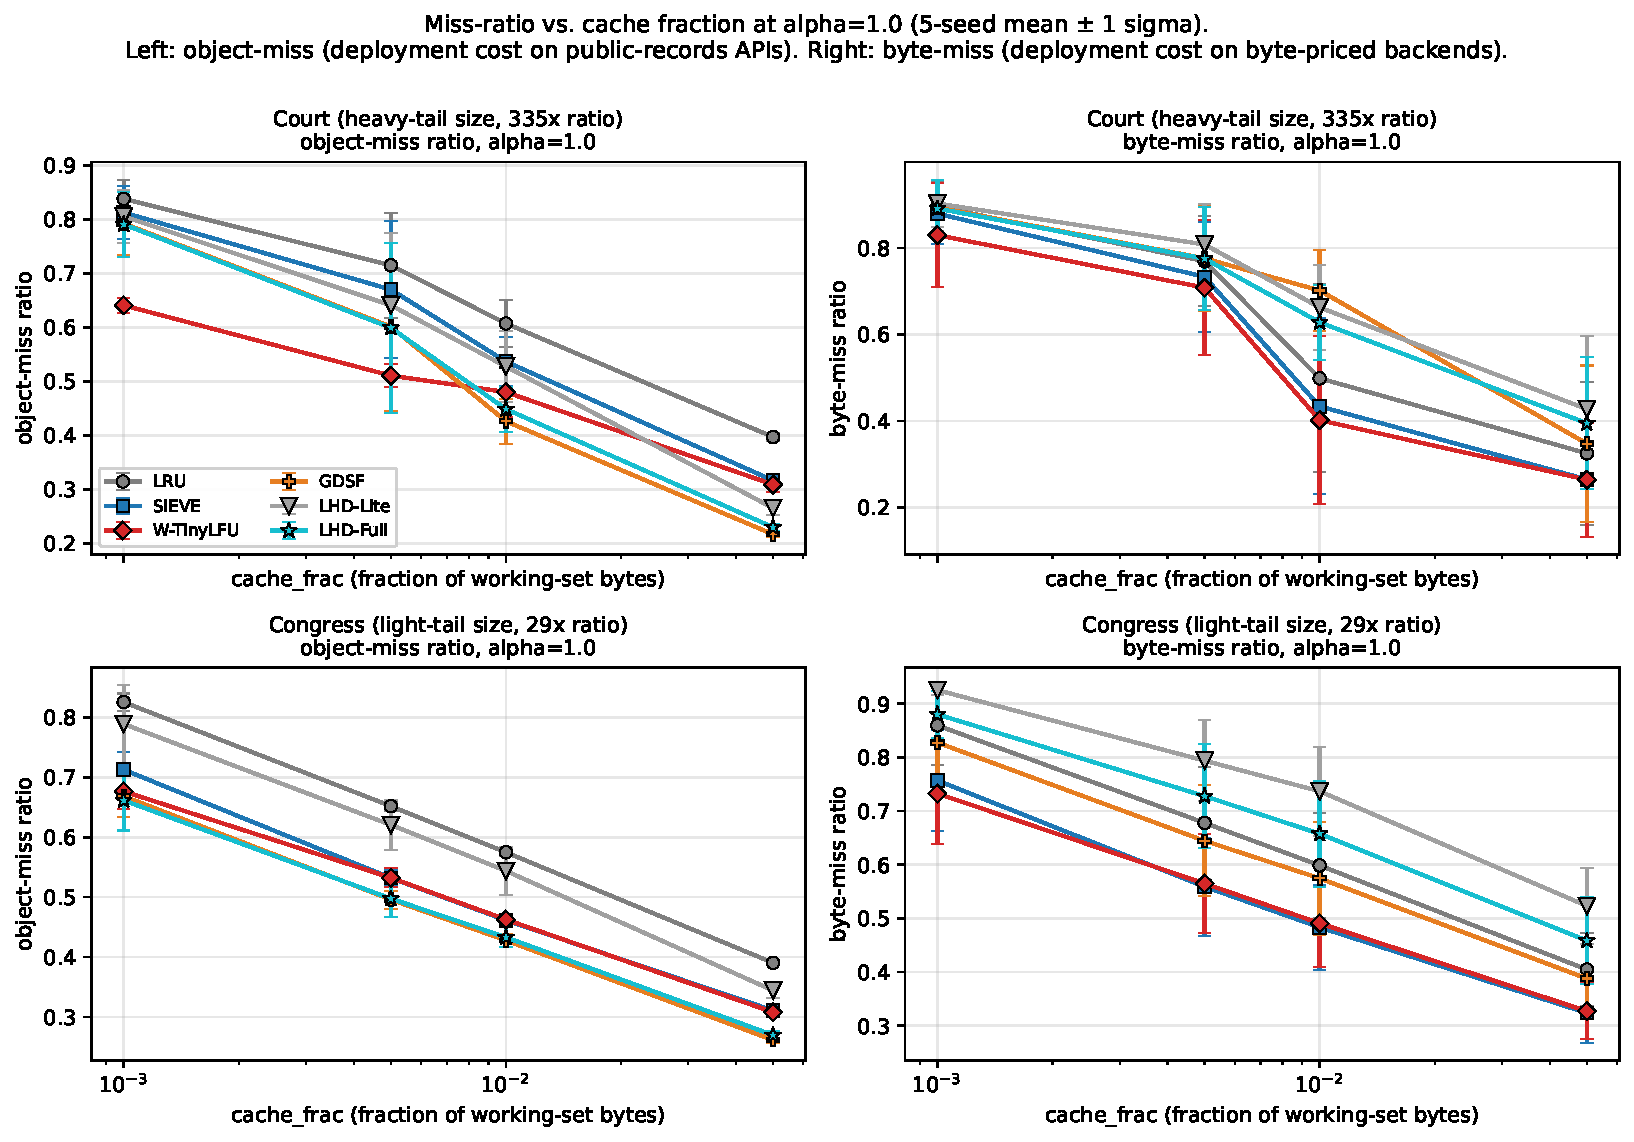
\includegraphics[width=0.95\textwidth]{figures/miss_vs_cf.pdf}
\caption{Miss-ratio vs.\ cache fraction at $\alpha = 1.0$, $5$-seed
mean $\pm 1\sigma$. \textbf{Court (top):} W-TinyLFU leads object-miss
at $\code{cf} \leq 0.005$; GDSF and LHD-Full overtake at $\geq 0.01$
(the Table~\ref{tab:focal-court} crossover, plotted). \textbf{Congress
(bottom):} GDSF and LHD-Full are visually indistinguishable on
object-miss; SIEVE/W-TinyLFU lead byte-miss.}
\label{fig:miss-vs-cf}
\end{figure*}

\paragraph{Congress focal.} On Congress, the object-miss winner
depends on $\alpha$ (Figure~\ref{fig:congress-alpha}):

\begin{table}[t]
\centering
\footnotesize
\renewcommand{\arraystretch}{0.9}
\begin{tabularx}{\columnwidth}{@{}lXXXXl@{}}
\toprule
$\alpha$ & SIEVE & W-TLFU & GDSF & LHD-F & winner \\
\midrule
$0.6$ & $0.873$ & $0.872$ & $0.850$ & $\mathbf{0.831}$ & LHD-F \\
$0.8$ & $0.707$ & $0.709$ & $0.675$ & $\mathbf{0.670}$ & LHD-F \\
$1.0$ & $0.461$ & $0.463$ & $\mathbf{0.428}$ & $0.433$ & GDSF \\
$1.2$ & $0.243$ & $0.245$ & $\mathbf{0.218}$ & $0.226$ & GDSF \\
\bottomrule
\end{tabularx}
\caption{Congress object-miss at $\code{cache\_frac} = 0.01$, all
four $\alpha$. LHD-Full's residual-reuse-distance beats GDSF's
size-priority at low $\alpha$ (weak frequency signal); GDSF wins at
high $\alpha$. Pattern holds across cf $\in \{0.005, 0.01, 0.05\}$.
\textbf{Power caveat:} the $\alpha=0.6$ gap ($1.9$\,pp) is robust at
$5$ seeds; the $\alpha=0.8$ gap ($0.5$\,pp) is comparable to
seed-$\sigma$ ($0.4$--$0.7$\,pp pooled across the four policies) and
was \emph{not} re-checked at $20$ seeds, unlike the Congress
SIEVE-vs.-W-TinyLFU power check in \S\ref{sec:mechanism}; treat the
$\alpha=0.8$ result as suggestive, not confirmed.}
\label{tab:focal-congress}
\end{table}

\begin{figure}[t]
\centering
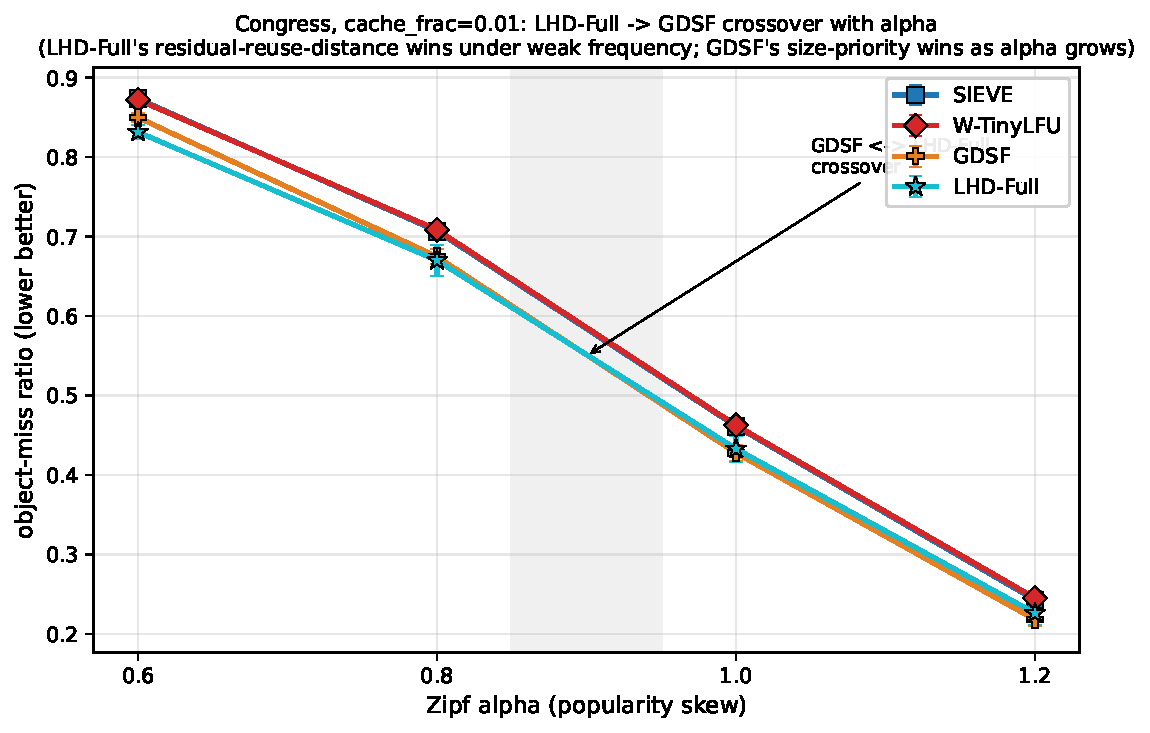
\includegraphics[width=0.95\columnwidth]{figures/congress_alpha_crossover.pdf}
\caption{Congress object-miss vs.\ $\alpha$ at $\code{cf}=0.01$
(Table~\ref{tab:focal-congress} plotted). LHD-Full leads at
$\alpha \in \{0.6, 0.8\}$; GDSF takes over at $\alpha \geq 1.0$.
SIEVE and W-TinyLFU are indistinguishable (\S\ref{sec:mechanism},
$p \geq 0.20$ at $20$ seeds).}
\label{fig:congress-alpha}
\end{figure}

\paragraph{LHD-Full's actual position.} LHD-Full anchors the object-miss
frontier on Congress at low $\alpha$ (Table~\ref{tab:focal-congress},
Figure~\ref{fig:congress-alpha}) but on Court is dominated by the
GDSF--W-TinyLFU convex hull at deployment-relevant cache fractions
(per-cell breakdown \S\ref{sec:weighted}). The 2-D class
implementation closes a $7$\,pp gap vs.\ LHD-Lite at
$(\alpha, \text{cf}) = (1.0, 0.01)$; per
\S\ref{sec:methodology}'s Memcached-faithful validation, the
residual Court-side gap is workload-class divergence, not
implementation incompleteness. Throughput $\sim 500$\,K acc/sec,
$14\times$ slower than W-TinyLFU.

%-------------------------------------------------------------------------------
\section{Cost Attribution}\label{sec:weighted}
%-------------------------------------------------------------------------------

\noindent \emph{Pick the metric that matches the operator's binding
cost.} The two metrics in $\S$\ref{sec:gdsf} disagree; most cache
benchmarks resolve this by silently picking object-miss (Memcached-
style) or byte-miss (CDN-style). I make the cost model explicit and
let it select a Pareto-frontier point.

\paragraph{Worked example: a $5.4$\,pp object-miss saving in operator
units.} Take the GDSF-vs.-W-TinyLFU gap at $(\alpha, \text{cf}) =
(1.0, 0.01)$ on Court: $0.480 \to 0.426 = 5.4$\,pp. Translate to
operator-binding-cost in three steps.

\textit{(i) Rate-limit headroom.} Origin reqs/hr $=
\text{object-miss} \cdot R_{\text{offered}}$. At an offered load of
$18{,}000$ reqs/hr (a modest civic-tech deployment with a few hundred
concurrent users), GDSF issues $7{,}668$ origin reqs/hr vs.\
W-TinyLFU's $8{,}640$ — a $972$ req/hr saving. Against the
$5{,}000$ reqs/hr quota that scales linearly: at $18{,}000$ offered,
both policies are still over quota and the $972$/hr saving is the
difference between needing $1.7$ API keys (GDSF) and $1.9$ keys
(W-TinyLFU) — i.e., the marginal user the operator can serve before
spinning up another credentialed pool. At $50{,}000$/hr offered the
saving is $2{,}700$/hr, which is half a quota slot.

\textit{(ii) End-user latency.} Per-request latency at
$L_{\text{origin}} = 383$\,ms drops from $184$\,ms (W-TinyLFU) to
$163$\,ms (GDSF), a $\sim 21$\,ms saving per request
(Table~\ref{tab:lat}). Across $20$\,K requests/day that is
$\sim 7$\,minutes of aggregate user wait time eliminated daily.

\textit{(iii) Byte-miss is zero deployment cost here.} GDSF's
byte-miss is $30$\,pp \emph{worse} than W-TinyLFU's ($0.702$ vs.\
$0.402$). For a public-records operator: zero dollars, zero
rate-limit budget. Bytes are free; requests are scarce. This is the
attribution decision that flips the policy verdict.

\paragraph{Public-records cost model.} The operator pays for
requests issued to origin (rate-limit budget), end-user latency
(proportional to object-miss given TTFB-dominated origin), and
origin server load (reputational); all three scale with object-miss,
none with bytes. Byte-miss is a diagnostic, not a deployment cost on
this workload class.

\paragraph{Latency $\approx$ object-miss $\cdot L_{\text{origin}}$
holds at realistic throughputs.} For a steady-state cache:
$\mathbb{E}[\text{lat}] = H \cdot L_{\text{cache}} + (1-H) \cdot
L_{\text{origin}}$. Take the $462$\,KB Court outlier as worst-case
transfer: at $10$\,MB/s WAN it is $46$\,ms vs.\ $L_{\text{origin}} =
358$\,ms ($13\%$); for typical $12$\,KB objects, $1.2$\,ms. The
approximation holds within $5$\,pp up to $\sim 100$\,KB. Origin TTFB
is dominated by backend-database response time (CourtListener built
on RECAP infrastructure; Congress.gov on the Library of Congress's
record system); not optimizable from the cache layer.
Table~\ref{tab:lat} translates the per-policy object-miss into
per-request latency at the Court anchor.

\begin{table}[t]
\centering
\footnotesize
\renewcommand{\arraystretch}{0.95}
\begin{tabularx}{\columnwidth}{@{}lXXX@{}}
\toprule
\textbf{Court @ cf $= 0.01$, $\alpha = 1.0$} & \textbf{obj-miss} & \textbf{lat/req (ms)} & \textbf{vs.\ no-cache} \\
\midrule
no cache  & $1.000$        & $383$ & $1.00\times$ \\
LRU       & $0.607$        & $233$ & $0.61\times$ \\
SIEVE     & $0.537$        & $206$ & $0.54\times$ \\
LHD-Lite  & $0.528$        & $203$ & $0.53\times$ \\
W-TinyLFU & $0.480$        & $184$ & $0.48\times$ \\
LHD-Full  & $0.449$        & $172$ & $0.45\times$ \\
GDSF      & $\mathbf{0.426}$ & $\mathbf{164}$ & $\mathbf{0.43\times}$ \\
\bottomrule
\end{tabularx}
\caption{Per-request latency, Court anchor $L_{\text{origin}} = 383$\,ms,
$L_{\text{cache}} = 1$\,ms. GDSF saves $\sim 21 / 39 / 69$\,ms vs.\
W-TinyLFU / LHD-Lite / LRU.}
\label{tab:lat}
\end{table}

\paragraph{Byte-miss variance.} Byte-miss has $4$--$7\times$ the
seed-$\sigma$ of object-miss on Court (W-TinyLFU $0.402 \pm 0.241$,
std/mean $= 60\%$): a single realization either samples the heavy
outlier into cache or doesn't, and the answer flips $\sim 30$\,pp.
This is why I don't decide the headline on byte-miss.

\paragraph{Why GDSF wins object-miss at mid-cache, W-TinyLFU at small
cache.} At $\code{cache\_frac} = 0.01$ on Court ($\sim 596$\,KB byte
budget; $\sim 50$ items if cached at the $E[\text{size}]=12$\,KB
average, $\sim 430$ if biased toward small items), GDSF refuses to
admit the $462$\,KB document, freeing roughly $230 \cdot$ a $2$\,KB
item or $2{,}300 \cdot$ a $200$\,B stub into cache
(\S\ref{sec:gdsf}'s priority math); the document is fetched on every
visit. W-TinyLFU's CMS instead admits the document if its frequency
exceeds incumbents', keeping it in cache and crowding out small
items. At small cache ($\code{cache\_frac} \leq 0.005$, $\sim
298$\,KB, can't even fit the outlier), the budget admits only the
very hottest items; GDSF's size-priority then crowds out
big-but-frequent items in favor of small mid-frequency items, which
hurts object-miss; W-TinyLFU's frequency-only admission wins. The
crossover at $\code{cache\_frac} \in [0.005, 0.01]$ is robust across
$\alpha \in \{0.6, 0.8, 1.0, 1.2\}$ on Court.

\paragraph{LHD-Full is Pareto-dominated on Court where caching matters.}
Worked example at $(\alpha, \text{cf}) = (1.0, 0.01)$: GDSF $(0.426,
0.702)$, W-TinyLFU $(0.480, 0.402)$, LHD-Full $(0.449, 0.628)$. The
convex combination at byte $= 0.628$ has $t = 0.247$, giving
$\text{obj} = 0.439$, $1$\,pp better than LHD-Full at the same
byte-miss. Per-cell check (Table~\ref{tab:lhdfull-pareto}):
\textbf{Pareto-dominated in $8/16$ Court cells} (including $7/8$
deployment-relevant cells at $\code{cache\_frac} \geq 0.01$ by
$0.5$--$3.6$\,pp); Pareto-\emph{in}comparable in the other 8
(byte-miss outside the GDSF--W-TinyLFU interval). LHD-Full never
strictly beats either endpoint on both axes. LHD-Full's
$14\times$ throughput penalty therefore buys nothing measurable.

\begin{table}[t]
\centering
\footnotesize
\renewcommand{\arraystretch}{0.95}
\begin{tabularx}{\columnwidth}{@{}lXXXX@{}}
\toprule
$\Delta_{\text{obj}}$ (pp)
& cf $0.001$ & cf $0.005$ & cf $0.01$ & cf $0.05$ \\
\midrule
$\alpha = 0.6$ & --- & --- & $\mathbf{+1.4}$ & $\mathbf{+1.4}$ \\
$\alpha = 0.8$ & --- & --- & $\mathbf{+3.6}$ & $\mathbf{+3.0}$ \\
$\alpha = 1.0$ & --- & --- & $\mathbf{+0.9}$ & $\mathbf{+1.3}$ \\
$\alpha = 1.2$ & --- & $\mathbf{+0.0}$ & --- & $\mathbf{+0.5}$ \\
\bottomrule
\end{tabularx}
\caption{Per-cell Pareto gap: positive $\Delta_{\text{obj}}$ means the
GDSF$\to$W-TinyLFU convex line achieves lower object-miss than LHD-Full
at LHD-Full's byte-miss (LHD-Full above the convex line). \textbf{Bold} = Pareto-dominated; dashed =
incomparable (LHD-Full's byte-miss outside the convex-hull range).
The $+0.0$ and $+0.5$\,pp gaps at $\alpha = 1.2$ sit within byte-miss
seed-$\sigma$ (could flip with more seeds); the $\geq +1.3$\,pp gaps
at lower $\alpha$ are robust.}
\label{tab:lhdfull-pareto}
\end{table}

\paragraph{Aside: byte-priced backends flip the verdict.} For
deployments where the operator pays per-byte (S3 pricing: $\$0.0004
/ 1{,}000$ requests $+ \$0.09 /$ GB egress; egress applies only to
cross-region or out-of-AWS traffic, not same-region S3-to-EC2),
W-TinyLFU's byte-miss advantage drives $\sim 32\%$ total-dollar
saving on Court at $\code{cache\_frac}=0.01$ (request and egress
costs combined, egress dominant): same measurements, opposite
verdict. The metric choice is not theory-neutral; it tracks who pays.

%-------------------------------------------------------------------------------
\section{Mechanism: Size-Outlier Rejection on Court, Ties on Congress}\label{sec:mechanism}
%-------------------------------------------------------------------------------

The SIEVE-vs.-W-TinyLFU gap on Court is $3.6$--$6.2$\,pp at
$\code{cache\_frac} = 0.01$ across $\alpha$ (smallest at $\alpha=1.2$). I initially predicted
this would track frequency-gradient richness (W-TinyLFU's CMS captures
gradient; SIEVE's visited-bit doesn't). Three ablations falsify that.

\begin{table*}[t]
\centering
\footnotesize
\renewcommand{\arraystretch}{0.95}
\begin{tabularx}{\textwidth}{@{}lXXXX@{}}
\toprule
$\alpha$ & full Court & strip $75$ size $> 100$\,KB & strip $20$ keys with freq $\geq 10$ & strip $75$ random 1-access (mean of 5) \\
\midrule
$0.6$ & $+4.4 \pm 0.7$\,pp & $+1.7 \pm 0.4$\,pp ($-62\%$) & $+5.1 \pm 0.7$\,pp ($+16\%$) & $+4.5 \pm 0.2$\,pp ($-2\%$) \\
$0.8$ & $+6.2 \pm 0.7$\,pp & $+1.4 \pm 0.4$\,pp ($-78\%$) & $+6.2 \pm 0.6$\,pp ($-1\%$) & $+5.6 \pm 0.4$\,pp ($+9\%$) \\
$1.0$ & $+5.6 \pm 0.8$\,pp & $+1.7 \pm 0.7$\,pp ($-71\%$) & $+5.5 \pm 1.4$\,pp ($-3\%$) & $+5.3 \pm 0.5$\,pp ($+6\%$) \\
$1.2$ & $+3.6 \pm 1.0$\,pp & $+1.3 \pm 0.1$\,pp ($-65\%$) & $+3.8 \pm 1.0$\,pp ($+6\%$) & $+3.8 \pm 0.5$\,pp ($-6\%$) \\
\bottomrule
\end{tabularx}
\caption{Three controls on the SIEVE $-$ W-TinyLFU gap (Court,
$\code{cache\_frac} = 0.01$). \textbf{Size-strip:} $62$--$78\%$
shrinkage. \textbf{High-freq strip} (zero size overlap): $\sim 0\%$.
\textbf{Matched-cardinality random 1-access strip} (75 keys, 75 rows
matched to size-strip): $\sim 0\%$. The shrinkage is specifically
about size-outliers, not key-cardinality and not access-concentration.}
\label{tab:mechanism-decomp}
\end{table*}

\paragraph{Mechanism, narrowed.} Both SIEVE and W-TinyLFU use
frequency-based eviction signals; neither is explicitly size-aware.
The structural difference is \emph{when} the frequency check runs.
W-TinyLFU's filter is pre-admission: a newcomer's CMS estimate is
compared to the incumbent's CMS, and the newcomer is refused if it
loses. SIEVE's filter is post-admission: every key is admitted, and
the visited-bit sweep evicts whatever wasn't re-touched.

On a heavy-tailed size distribution where rare-large items arrive,
this asymmetry compounds. W-TinyLFU rejects the $462$\,KB Court
opinion outright. SIEVE admits it; before the next visited-bit
sweep can evict it, that single admission has cascade-evicted
$\sim 230$ small items ($\sim 2$\,KB displaced-item average; the
ratio scales as $1/E[\text{size}]_{\text{small}}$). Each of those
$230$ small items is now a guaranteed future miss. \emph{Those
cascade evictions are the gap.}

\paragraph{Why the matched-cardinality control is load-bearing.}
Reading Table~\ref{tab:mechanism-decomp} left-to-right: the
size-strip column ($-62$ to $-78\%$ shrinkage) and the high-freq
strip column ($\sim 0\%$) are the obvious decomposition — strip
size-outliers and the gap collapses; strip 20 keys that happen to
have high frequency but no size overlap and the gap stays. A skeptic
could still object: ``you removed $75$ keys in the size-strip; maybe
SIEVE is just unlucky on some property correlated with cardinality.''
The third column rules that out. \textbf{Strip $75$ random 1-access
keys (matched cardinality, no size correlation): $\sim 0\%$
shrinkage} ($-2$\,\% to $+9$\,\%, all within seed-$\sigma$).
Removing equivalent cardinality without removing the heavy-size tail
does not move the gap. Only the size-tail removal does.

The triangulation is what makes the size-outlier mechanism a finding
rather than a guess: the obvious strip identifies a candidate; the
high-freq strip rules out the alternative ``it's just a hot key'';
the matched-cardinality strip rules out ``it's just $75$ keys.'' The
mechanism is therefore \emph{frequency-aware pre-admission filtering
on heavy-tailed size distributions}, and the size-outlier sensitivity
is emergent from how admission gating interacts with size variance —
not size-awareness in either policy. This is what falsified my
initial frequency-gradient hypothesis.

\paragraph{Power check.} The SIEVE-vs.-W-TinyLFU object-miss gaps
on Congress at $\code{cache\_frac}=0.01$ are tiny: $0.1$--$0.3$\,pp
across $\alpha \in \{0.6, 0.8, 1.0, 1.2\}$, with pooled seed
$\sigma \approx 0.8$--$1.3$\,pp (gap/$\sigma$ ratios $0.1$--$0.2$).
Re-running at $20$ seeds with Welch's $t$-test confirms all $p \geq
0.20$. The original 5-seed result was not underpowered for an effect
of this size; SIEVE and W-TinyLFU are genuinely indistinguishable on
Congress object-miss.

%-------------------------------------------------------------------------------
\section{Ablations}\label{sec:ablations}
%-------------------------------------------------------------------------------

Four ablations close the methodological loop. \textbf{S3-FIFO
small-queue ratio:} smaller wins monotonically on heavy-tailed Court
synthetic ($\alpha=1.2$), $5\%$ beats $20\%$ by $6.3$\,pp;
practitioners should reduce toward $5\%$ from Yang et al.'s $10\%$
recommendation. \textbf{SIEVE visited-bit:} toggling
\texttt{promote\_on\_hit} off loses by $+15.4$\,pp on Congress at
$\alpha=1.0$, the largest single-toggle delta in the study,
empirically confirming the NSDI'24 claim. \textbf{W-TinyLFU $\pm$
Doorkeeper:} null result, Congress within $\pm 0.22$\,pp and Court
direction-swaps at $\alpha$ extremes — cannot distinguish ``no real
effect'' from ``no detectable effect at $20$\,K trace.''
\textbf{SHARDS~\cite{waldspurger2015shards}:} self-convergence on a
$1$\,M synthetic ($\alpha=0.8$) gives $1\%$-vs.-$10\%$ MAE $=0.038$,
passing the $<0.05$ sanity gate; a $50$\,K oracle regime with exact
stack distances reproduces the convergence.

%-------------------------------------------------------------------------------
\section{Conclusion}\label{sec:conclusion}
%-------------------------------------------------------------------------------

The object-miss winner is workload-shape-dependent: GDSF on Court at
$\code{cache\_frac} \geq 0.01$ and Congress at $\alpha \geq 1.0$;
LHD-Full on Congress at $\alpha \leq 0.8$; W-TinyLFU on Court at
$\code{cache\_frac} \leq 0.005$. What is interesting is \emph{why}
the GDSF result has been absent from the post-2020 cache literature,
and why ``just apply a modern policy to API caching'' gives the
wrong answer.

\paragraph{What this contributes.} The core move is
workload-class-specific cost attribution: modern cache papers each
pick one metric matching their target
(SIEVE~\cite{zhang2024sieve}, S3-FIFO~\cite{yang2023fifo},
ARC~\cite{megiddo2003arc}: object-miss; LHD~\cite{beckmann2018lhd}:
byte-miss for CDN), so operators outside that target cannot read off
a deployment answer. Making the cost model explicit
(\S\ref{sec:weighted}) flips the answer between request-priced and
byte-priced backends on the same measurements — the metric you
choose is the policy you choose.

\paragraph{Limitations.} (a) Native-popularity trace: the
replay-Zipf overlay has not been compared against actual user traffic; an in-the-wild user population
might produce a distribution I did not test. (b) Byte-for-byte
LHD reference-code comparison (\S\ref{sec:methodology}): the
qualitative ranking is established (LHD-Full beats LRU $13$--$18$\,pp
on the Memcached-faithful synth, matches GDSF $\pm 0.5$\,pp), but
absolute-pp agreement against the CMU-CORGI/LHD simulator is not yet
checked. (c) Third-domain test (SEC EDGAR has
the same rate-limit + size-variance structure with a different
access pattern).

\paragraph{Practitioner rule (public-records APIs only).}
\begin{itemize}[leftmargin=*,itemsep=1pt,topsep=1pt]
  \item \textbf{Heavy-tail size} (Court-like, $462$\,KB outliers in
    catalog): \textbf{GDSF} at $\code{cache\_frac} \geq 0.01$ (saves
    $\sim 21$\,ms/request at Court's $L_{\text{origin}}=383$\,ms,
    $\sim 970$ origin reqs/hr at $18{,}000$/hr offered);
    \textbf{W-TinyLFU} at $\code{cache\_frac} \leq 0.005$ (GDSF's
    size-priority crowds out big-but-frequent items).
  \item \textbf{Light-tail size} (max/median $\ll$ Court's $335\times$;
    Congress at $29\times$): \textbf{LHD-Full} at $\alpha \leq 0.8$
    (residual-reuse-distance beats size-priority when frequency is
    weak, $0.5$--$2$\,pp; $\alpha=0.8$ within seed-$\sigma$ at $5$
    seeds, treat as suggestive); \textbf{GDSF} at $\alpha \geq 1.0$.
  \item Throughput: GDSF $\approx$ W-TinyLFU $\approx 7$\,M acc/sec;
    LHD-Full $14\times$ slower, but on Congress at low $\alpha$ it
    is the only policy that wins. Byte-priced backends:
    W-TinyLFU on Court (heavy-tail), SIEVE on Congress (light-tail,
    $12/16$ cells); see \S\ref{sec:weighted}.
\end{itemize}

\paragraph{When does this generalize?} The framework — \emph{pick
the metric that matches the operator's binding cost; the policy
follows} — applies to any workload class with four traits:
(1)~\textbf{per-request origin cost, not per-byte} (rate-limited
APIs, monetary quotas, scrape-respectful crawlers); (2)~\textbf{TTFB-
dominated origin} (RTT $\gg$ payload/bandwidth, so latency
$\approx$ object-miss $\times L_{\text{origin}}$); (3)~\textbf{heavy
size variance within a single key namespace} (not size-binned by
content type — this is what makes GDSF's size-priority discriminate
between co-mingled items rather than ratifying a routing decision);
(4)~\textbf{heavy-tailed popularity ($\alpha \gtrsim 1$)} so
cache-fraction sensitivity doesn't drown out policy choice.
\textbf{SEC EDGAR} is the obvious next datapoint: traits (1)--(3)
match Court closely (rate-limit, government back-end, 10-K vs.\ 8-K
size variance); trait (4) is uncertain because EDGAR access tends to
be filing-targeted rather than catalog-then-deepdive. Conjecture:
GDSF wins object-miss at $\code{cache\_frac} \geq 0.01$ on
size-variant filings, with the GDSF--W-TinyLFU crossover at a larger
cache fraction than Court since EDGAR's frequency tail is weaker.
Confirming would establish workload-class cost attribution as the
default framing rather than a single-domain artifact.

%-------------------------------------------------------------------------------
\section*{Availability}
%-------------------------------------------------------------------------------

Source code, traces, and experimental results are available at the
project repository.

%-------------------------------------------------------------------------------
\begin{thebibliography}{99}
%-------------------------------------------------------------------------------
\scriptsize
\setlength{\itemsep}{0pt}
\setlength{\parsep}{0pt}

\bibitem{einziger2017tinylfu} Einziger et al. \textit{TinyLFU.} ACM TOS, 2017.
\bibitem{caffeine2024} Manes, B. \textit{Caffeine: high-performance Java caching library.} \url{https://github.com/ben-manes/caffeine}, 2014--present.
\bibitem{yang2023fifo} Yang et al. \textit{FIFO queues are all you need for cache eviction.} SOSP, 2023.
\bibitem{zhang2024sieve} Zhang et al. \textit{SIEVE is simpler than LRU.} NSDI, 2024.
\bibitem{waldspurger2015shards} Waldspurger et al. \textit{Efficient MRC construction with SHARDS.} FAST, 2015.
\bibitem{clauset2009powerlaw} Clauset, Shalizi, Newman. \textit{Power-law distributions in empirical data.} SIAM Rev.\ 51(4), 2009.
\bibitem{cherkasova1998gdsf} Cherkasova. \textit{Improving WWW Proxies Performance with GDSF.} HPL-98-69 (R.1), 1998.
\bibitem{beckmann2018lhd} Beckmann, Chen, Cidon. \textit{LHD: maximizing hit density.} NSDI, 2018.
\bibitem{megiddo2003arc} Megiddo, Modha. \textit{ARC: self-tuning, low-overhead replacement cache.} FAST, 2003.

\end{thebibliography}

\end{document}